\documentclass[12pt,a4paper]{article}
\usepackage[utf8]{inputenc} %polskie znaki
\usepackage[T1]{fontenc}	%polskie znaki
\usepackage{amsmath}		%matematyczne znaczki :3
\usepackage{enumerate}		%Dodatkowe opcje do funkcji enumerate
\usepackage{geometry} 		%Ustawianie marginesow
\usepackage{graphicx}		%Grafika
\usepackage{wrapfig}		%Grafika obok textu
\usepackage{float}			%Allows H in fugire
\pagestyle{empty} 			%usuwa nr strony

\newgeometry{tmargin=2cm, bmargin=2cm, lmargin=2cm, rmargin=2cm} 

\begin{document}
	\begin{center}
		\LARGE Rachunek prawdopodobieństwa i stereometria - test
	\end{center}
	\vspace{1.5cm}
	\begin{flushright}
		\textbf{1 TERMIN}
	\end{flushright}
	\begin{tabular}{p{13cm} r}
		Imię i nazwisko: ............................................................................
		&[....../30pkt]\\ 
		\vspace{0.5cm}
	\end{tabular}
	\begin{enumerate}[1.]
		\item  \begin{tabular}{p{13cm} r}
			Oblicz ile jest liczb  8-cyfrowych, które są podzielne przez 5, trzecia, czwarta i piąta cyfra jest taka sama, a wszystkie pozostałe są różne między sobą.&[3pkt]\\ 
		\end{tabular}
		
		\item  \begin{tabular}{p{13cm} r}
			Do kina planuje się wybrać 10 osób, w tym Marek i Ewa. Otrzymali miejsca tak ja na rysunku poniżej.&[4pkt]\\ 
		\end{tabular}
		
		\begin{figure}[h]
			\centering
			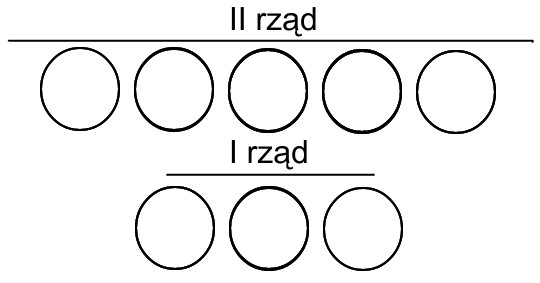
\includegraphics[scale=0.4]{rpst1.jpeg}
		\end{figure}
		
		Oblicz na ile sposobów mogą usiąść te osoby:
		\begin{enumerate}[a)]
			\item dowolnie
			\item tak aby Marek i Ewa siedzieli obok siebie.
			\item tak aby Marek i Ewa byli w 2 rzędzie.
			\item tak aby Marek i Ewa siedzieli w różnych rzędach.
		\end{enumerate}
		
		\item  \begin{tabular}{p{13cm} r}
			Grupa znajomych ogarnanizowała imprezę, na której mają puścić 4 filmy. Wybrali się do wyporzyczalni filmów, gdzie sprzedawca zaproponował im 20 różnych filmów. Na ile sposobów mogą wygrać filmy na tę imprezę?&[2pkt]\\ 
		\end{tabular}
		
		\item  \begin{tabular}{p{13cm} r}
			Oblicz prawdopodobieństwo, że w dwukrotnym rzucie siedmościenną kostką do gry, suma oczek będzie parzysta.&[3pkt]\\ 
		\end{tabular}
		
		\item  \begin{tabular}{p{13cm} r}
			Tata Krzyśka to fanatyk wędkarstwa. Niestety jego tata często zostawia haczyki na podłodze i przez to wbija sobie je do nogi. Szansa na to, że danego dnia Krzyś wbije sobie haczyka wynosi zawsze 10\%. Oblicz prawdopodobieństwo, że Krzyś w ciągu tygodnia nie wbije sobie haczyka do nogi. &[3pkt]\\ 
		\end{tabular}
		
		\item  \begin{tabular}{p{13cm} r}
			Oblicz medianę, dominantę i średnią arytmetyczną ocen testów studentów z tabeli &[3pkt]\\ 
		\end{tabular}
		
		\begin{tabular}{|c|c|c|c|c|c|}
			\hline
			Ocena&1&2&3&4&5\\
			\hline
			Liczba studentów&20&20&30&50&20\\
			\hline
		\end{tabular}
		\newpage
		\item  \begin{tabular}{p{13cm} r}
			Dany jest graniastosłup prawidłowy sześciokątny o krawędzi podstawy 4 i najdłuższej przekątnej równej 16. Oblicz jego:&[6pkt]\\ 
		\end{tabular}
		\begin{enumerate}[a)]
			\item objętość
			\item pole powierzchni całkowitej
			\item sinus kąta między przekątną ściany bocznej a krawędzią podstawy
		\end{enumerate}
		
		\item  \begin{tabular}{p{13cm} r}
			Dany jest ostrosłup prawidłowy czworokątny, którego wszystkie krawędzie są tej samej długości, a ich suma wynosi 32. Oblicz jego:&[6pkt]\\ 
		\end{tabular}
		\begin{enumerate}[a)]
			\item objętość
			\item pole powierzchni całkowitej
		\end{enumerate}
		
		
		
	\end{enumerate}
	
\end{document}
